\section{РУКОВОДСТВО ПОЛЬЗОВАТЕЛЯ}
\label{sec:manual}

\def\dc{Docker}

В данном разделе будет описана последовательность действий, которую необходимо произвести пользователям для использования данного программного продукта.

Сам продукт распространяется в качестве проекта с открытым исходным кодом по лицензии Apache License.
Это означает, что каждый желающий может присоединиться к разработке и дальнейшему развитию проекта.

По этой причине, важную часть проекта также занимает документация и инструменты непрерывной интеграции.

Данный проект может использоваться как отдельная программа в локальной системе, либо в качестве компонента более масштабной системы.
По этой причине продукт можно сконфигурировать под разные окружения.

Основные режимы работы:
\begin{itemize}
    \item Локальный режим;
    \item Режим кластера.
\end{itemize}

\subsection{Руководство для локального режима}

Данное руководство предназначено для локальной развёртки приложения и работы на одной машине.

\subsubsection{Требования к программному обеспечению}

Для корректной сборки и работы данного дипломного проекта требуется следующее программное обеспечение:
\begin{itemize}
    \item Docker-compose версии выше 1.10.0+ (поддерживающий API версии 2.0);
    \item любой веб-браузер.
\end{itemize}

Для работы продукта в локальном режиме будет достаточно вышеперечисленного программного обеспечения.
Всё окружение, которое необходимо для работы компонентов системы обеспечивается с помощью Docker образов, а все компоненты системы работают в контейнере.

\subsubsection{Настройка рабочего окружения}

В первую очередь, необходимо установить docker-compose.
Инструкцию по установке данного инструмента для своей операционной системы можно найти на официальном сайте ~\cite{docker_compose_install_site}

Ниже приведён пример установки docker-compose для операционной системы Centos 7:

\begin{lstlisting}
$ export DOCKER_COMPOSE_VERSION='1.24.0'
$ sudo yum remove docker \
    docker-client \
    docker-client-latest \
    docker-common \
    docker-latest \
    docker-latest-logrotate \
    docker-logrotate \
    docker-engine
$ sudo yum install -y yum-utils \
    device-mapper-persistent-data \
    lvm2
$ sudo yum-config-manager \
    --add-repo \
    https://download.docker.com/linux/centos/docker-ce.repo
$ sudo yum install docker-ce docker-ce-cli containerd.io
$ sudo curl -L "https://github.com/docker/compose/releases/download/$DOCKER_COMPOSE_VERSION/docker-compose-$(uname -s)-$(uname -m)" -o /usr/local/bin/docker-compose
$ sudo chmod +x /usr/local/bin/docker-compose
$ sudo systemctl start docker
$ sudo usermod -aG docker $(whoami)
\end{lstlisting}

Для проверки корректности установки следует использовать следующие команды:

\begin{lstlisting}
$ docker run hello-world
$ docker-compose --version
\end{lstlisting}

Браузер необходим для взаимодействия с интерактивными документами.
Для примера возьмём установку браузера Mozilla Firefox для Linux:

\begin{lstlisting}
$ sudo yum install -y firefox    
\end{lstlisting}


После установки всех необходимых компонентов, можно приступить к запуску самого приложения.
Для получения приложения можно использовать DVD-диск, который идёт в комплекте к дипломному проекту, либо получить последнюю версию из GitHub:

\begin{lstlisting}
$ wget https://github.com/FyodorovAleksej/OpenAirPollutionMonitor/archive/master.zip
$ unzip ./OpenAirPollutionMonitor-master.zip
\end{lstlisting}

После получения проекта для начала необходимо установить необходимые настройки, либо использовать настройки по-умолчанию.
Для локального запуска подойдут настройки по-умолчанию.
Единственный параметр, который необходимо поменять - это указать свой API ключ для сервиса OpenWeatherMap.
Для его получения необходимо зарегистрироваться на этом сервисе и оформить подписку на используемый API ('').%TODO ADD AIR POLUTION API
После оформления подписки, на используемую почту придёт письмо с ключом.
Этот ключ необходимо вписать в файл конфигурации.
Эту операцию на Linux можно сделать следующим образом:

\begin{lstlisting}    
$ export OPEN_WEATHER_MAP_API_KEY="xxxxxxxxx"
$ sed -i -e "s/#YOUR_API_KEY#/$OPEN_WEATHER_MAP_API_KEY/g" ./src/OAPM/dumper/config/dumper_config.ini
\end{lstlisting}

После установки ключа, можно полноценно использовать приложение в локальном режиме.
Для этого можно использовать скрипт \texttt{startup.sh}.
Данный скрипт развернёт всё необходимое окружение для работы с помощью docker-compose.
Все компоненты приложения собираются в контейнеры, и запускаются в подготовленной среде.

В качестве готовых компонентов выступают следующие контейнеры:
\begin{itemize}
    \item Zookeeper;
    \item Apache Kafka;
    \item Apache Spark;
    \item Apache Zeppelin.
\end{itemize}

Zookeeper необходим для контроля kafka брокеров.
По-умолчанию он разворачивается в контейнере, и публикует порт 2181 наружу.
Это означает, что он доступен не только внутри созданной локальной подсети, но и с хоста.
Это позволяет отслеживать работу Zookeeper, и тем самым следить за работой kafka брокеров.

Apache kafka запускается в контейнере.
Так как kafka использует zookeeper для контроля брокеров, то необходимо задать адрес zookeeper сервера.
Docker-compose создаёт локальную подсеть, для связи всех контейнеров в собираемом файле, поэтому kafka контейнер будет находиться в одной сети с zookeeper.
Таким образом обеспечивается взаимосвязь между брокерами и zookeeper.

Для работы с kafka - публикуется порт 9092, с помощью которого можно подключиться и использовать топики.
Также сразу при создании контейнера запускается команда на создание топиков, которые необходимы приложению:
\begin{itemize}
    \item co-topic;
    \item so-topic;
    \item no-topic;
    \item oz-topic.
\end{itemize}

Apache Spark состоит из нескольких контейнеров:
\begin{itemize}
    \item master;
    \item worker 1;
    \item worker 2;
\end{itemize}

В разворачиваемом кластере должен быть один мастер узел, и сколько угодно рабочих узлов.
Как уже было упомянуто раньше, задача будет отправляться на мастер узел, а он в свою очередь распределит её на рабочие узлы, на которых задача будет выполняться параллельно.
Количество рабочих узлов при необходимости можно увеличить.

Apache Zeppelin представляет из себя аналог Jupyter.
При развёртке данного контейнера используется монтирование локальной директории, что позволяет сразу использовать заготовленные интерактивные документы.
Также для Zepelin указывается адрес spark-мастера.
Так как все контейнеры находятся в одной подсети - то указывается адрес созданного контейнера со spark-мастером.
Для подключения со стороны хоста - пробрасывается порт 8090.

Кроме вышеупомянутых сторонних контейнеров, также используется контейнер с самим приложением.
Он также монтируется к локальной системе, что позволяет использовать файлы хоста.
Такой принцип используется, чтобы можно было перезапускать данный контейнер и при этом не терять файлы, которые были получены с внешнего сервиса OpenWeatherMap.

После запуска всех необходимых контейнеров, для дальнейшей работы понадобится браузер.
Для этого необходимо перейти по адресу хоста, на котором развёрнуты все контейнеры через порт, который был опубликован для Apache Zeppelin.
По умолчанию - для Apache Zeppelin публикуется порт 8090.
Так как все эти контейнеры были развёрнуты на локальной машине, то необходимо перейти по адресу \texttt{localhost:8090}.
В случае, если Apache Zeppelin был успешно запущен, то при обращении по указанному адресу должна открыться страница, подобно той, что приведена на рисунке~\ref{pic:lit_manual:zeppelin_index}.

\begin{figure}
    \centering
    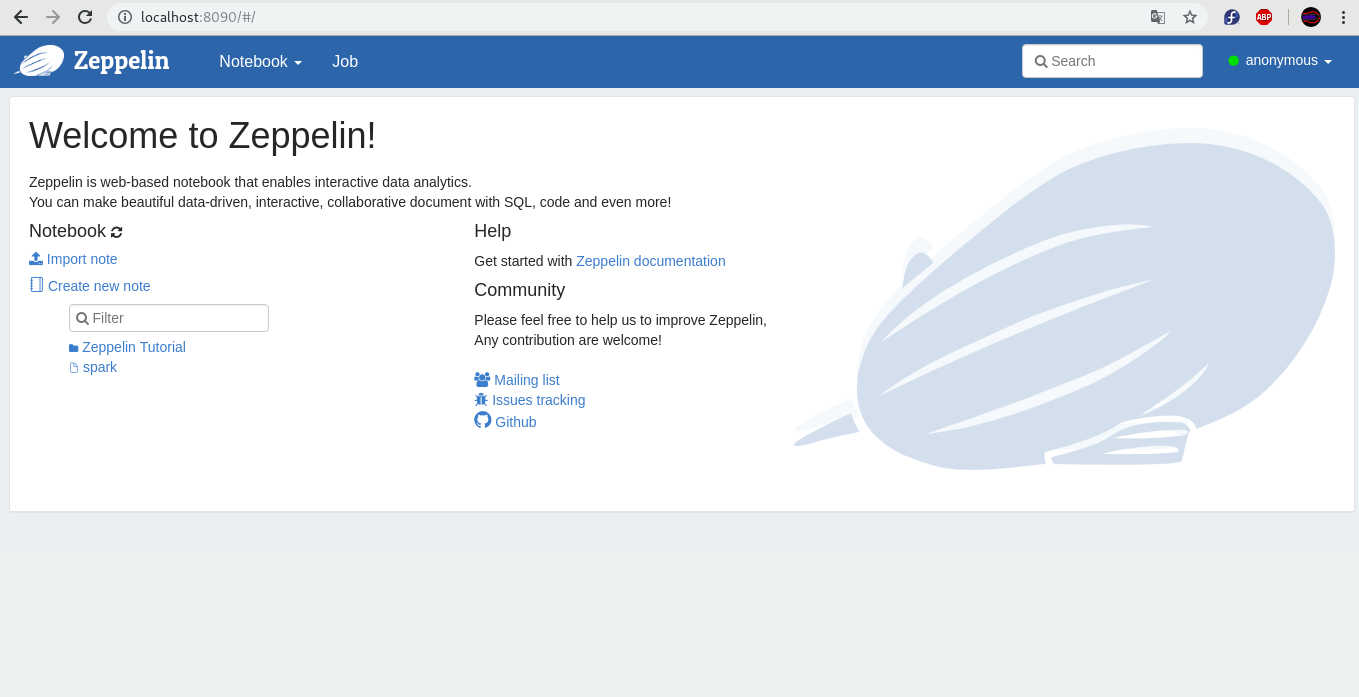
\includegraphics[width=0.7\textwidth]{zeppelin_index}
    \caption{Приветственная страница Apache Zeppelin}
    \label{pic:lit_manual:zeppelin_index}
\end{figure}

При открытии данной страницы, необходимо выбрать из предложенных интерактивных документов в списке \texttt{Notebooks}, документ с названием \texttt{spark}.
Когда откроется документ, остаётся только запустить его.
В случае, если Zeppelin попросит выбрать используемый интерпретатор, то необходимо выбрать \texttt{Spark}.

\subsection{Работа в режиме кластера}

Отличие в данном режиме заключается в том, что уже существует кластер, в котором есть все используемые компоненты.
Также в качестве подобного кластера может использоваться специальный образ (\texttt{sandbox}), который представляет из себя платформу Hadoop.

Например компании Cloudera и Hortonworks предоставляют подобный продукт.
В предоставляемом продукте уже существуют используемые компоненты.
Также в платформе Hadoop используется распределённая файловая система.
Разрабатываемый продукт как раз поддерживает работу с таким типом файловой системой.
Также из-за специфики распределения файлов, есть возможность создания Hive таблицы на скопированных данных.
Тем самым можно отслеживать используемые приложением файлы в системе.

В состав Hadoop платформы входят необходимые для разрабатываемого продукта компоненты:
\begin{itemize}
    \item Apache Zookeeper;
    \item Apache Kafka;
    \item Apache Spark;
    \item Apache Zeppelin.
\end{itemize}

В связи с этим отпадает потребность в локальном развёртывании вышеперечисленных компонентов.
В таком случае, необходимо установить необходимые адреса в файле конфигурации \texttt{./src/OAPM/dumper/config/dumper\_config.ini}.

Используемые топики должны быть созданы в используемом kafka брокере.

Для этого, необходимо выполнить следующую команду:
%TODO validate kafka command%
\begin{lstlisting}    
$ kafka-topics.sh --create-topic --partitions 1 --replication 1 --bootstrapserver localhost:6667 co-topic
\end{lstlisting}
Количество разделов и количество реплик необходимо устанавливать в соответствии с кластером.
Их количество обычно зависит от количества узлов данных в кластере.

Для проверки создания топиков необходимо использовать следующую команду:
\begin{lstlisting}
$ kafka-topics.sh --zookeeper zookeeper:2181 --list
\end{lstlisting}
В выводе команды должны быть указаны создаваемые топики.

Так как существует доступ ко всем необходимым компонентам системы, то можно запустить разрабатываемый продукт локально.
Для локального запуска потребуются следующие компоненты:

\begin{itemize}
    \item Python и pip версии 3.0 и выше;
\end{itemize}

Для запуска необходимо сначала установить все необходимые зависимости, которые приведены в файле \texttt{./src/OAPM/requirements.txt}.
Это можно сделать с помощью команды:
\begin{lstlisting}
$ sudo pip install -r ./src/OAPM/requirements.txt
\end{lstlisting}
Также вместо использования системного интерпретатора можно создать виртуальное окружение, и использовать его.
%TODO add venv

После утановки необходимых пакетов, достаточно запустить Python скрипт \texttt{./src/OAPM/dumper/cli.py}.
В качестве параметра данный скрипт принимает путь к файлу конфигурации.
Использует предоставляемый файл конфигурации \texttt{./src/OAPM/dumper/config/dumper\_config.ini} в качестве файла по-умолчанию.

После того, как приложение будет запущено, то можно использовать Apache Zeppelin.
Подключившись к нему, необходимо экспортировать интерактивный документ из файла \texttt{./src/docker/zeppelin/notebooks/spark/note.json}.
После экспортирования документа, необходимо открыть его и запустить.

